\documentclass[12pt,a4paper]{article}
\usepackage[utf8]{vietnam}
\usepackage{amsmath,amssymb}
\usepackage{tabularx}
\usepackage{tikz}
\usepackage{xcolor}
\usepackage[top=0.6cm, bottom=0.6cm, left=0.6cm, right=0.6cm]{geometry}
\usepackage[dethi]{ex_test}

\SAOPTN{widthSA=2.6,heightSA=0.62}
\setlength{\parskip}{0pt}

% Dong ke cham mo chuan viet tay
\newcommand{\dongke}[1]{%
  \begingroup%
  \setlength{\parskip}{0pt}%
  \baselineskip=18.5pt%
  \vspace{1.0mm}%
  \foreach \i in {1,...,#1}{%
    \noindent{\color{gray!60}\dotfill}\par%
  }%
  \vspace{0.6mm}%
  \endgroup%
}

% Dinh nghia o bai tap tu luan trong bang
\newcommand{\oBaiTap}[3][6]{%
  \vspace{1.0mm}%
  \noindent\textbf{#2} #3\par%
  \dongke{#1}%
}

\begin{document}
\pagestyle{empty}
% =============================================================================
% ========================= TOAN 9 TUAN 10 BUOI 01 - MA DE 101 =================
% ========================= TRANG 1/2 ==========================================
% =============================================================================
\noindent
\begin{tabularx}{\linewidth}{|X|c|}
\hline
\textbf{PHIẾU KIỂM TRA ĐỊNH KỲ TOÁN 9 - TUẦN 10 - BUỔI 1} & \textbf{Mã đề: 101 - Trang 1/2} \\
\hline
\end{tabularx}

\vspace{1.0mm}

\noindent
\begin{tabularx}{\linewidth}{|p{3.2cm}|X|}
\hline
\centering\textbf{ĐIỂM SỐ} & \centering\textbf{LỜI NHẬN XÉT CỦA THẦY CÔ} \tabularnewline
\hline
\rule{0pt}{1.8cm} & \tabularnewline
\hline
\end{tabularx}

\vspace{1.2mm}
\noindent\textbf{Câu 1 (0,25 điểm).} Cho $(O; 4\text{ cm})$, khoảng cách $d(O, a) = 4\text{ cm}$. Số điểm chung là: \shortans{1}\par\vspace{0.5mm}
\noindent\textbf{Câu 2 (0,25 điểm).} Tiếp tuyến $AB$ của $(O)$ tại tiếp điểm $B$. Số đo góc $\widehat{ABO}$ là: \shortans{90^\circ}\par\vspace{0.5mm}
\noindent\textbf{Câu 3 (0,25 điểm).} Cho $(O; 3\text{ cm}), OA = 5\text{ cm}$, tiếp tuyến $AB$ ($B \in (O)$). Độ dài $AB$ là: \shortans{4\text{ cm}}\par\vspace{0.5mm}
\noindent\textbf{Câu 4 (0,25 điểm).} Căn bậc hai số học của $121$ là: \shortans{11}\par\vspace{0.5mm}
\noindent\textbf{Câu 5 (0,25 điểm).} Điều kiện xác định của biểu thức $\sqrt{3x - 9}$ là: \shortans{x \ge 3}\par\vspace{0.5mm}
\noindent\textbf{Câu 6 (0,25 điểm).} Tính giá trị của biểu thức $\sqrt{32} - \sqrt{18} + \sqrt{8} = $ \shortans{3\sqrt{2}}\par\vspace{0.5mm}
\noindent\textbf{Câu 7 (0,25 điểm).} Hệ phương trình $\begin{cases} 2x + y = 7 \\ x - y = 2 \end{cases}$ có nghiệm $(x; y)$ là: \shortans{(3; 1)}\par\vspace{0.5mm}
\noindent\textbf{Câu 8 (0,25 điểm).} $\Delta$ vuông có đường cao $h$, hai hình chiếu $4\text{ cm}$ và $9\text{ cm}$. Độ dài $h$ là: \shortans{6\text{ cm}}\par\vspace{0.5mm}
\noindent\textbf{Câu 9 (0,25 điểm).} Đường tròn $(O; 5\text{ cm})$, dây $CD = 8\text{ cm}$. Khoảng cách từ $O$ đến $CD$ là: \shortans{3\text{ cm}}\par\vspace{0.5mm}
\noindent\textbf{Câu 10 (0,25 điểm).} Thang dài $4\text{ m}$, chân cách tường $2\text{ m}$. Góc tạo bởi thang và đất là: \shortans{60^\circ}\par\vspace{0.5mm}
\vspace{0.8mm}
\noindent\textbf{Câu 11 (2,5 điểm). Đại số tổng hợp:}
\vspace{0.6mm}

\noindent
\begin{tabularx}{\linewidth}{|X|X|}
\hline
\oBaiTap[19]{a) (1,25 điểm)}{Giải hệ phương trình: $\begin{cases} \dfrac{2}{x - 1} + \dfrac{1}{y + 2} = 4 \\ \dfrac{1}{x - 1} - \dfrac{2}{y + 2} = -3 \end{cases}$} & 
\oBaiTap[19]{b) (1,25 điểm)}{Cho $P = \left( \dfrac{\sqrt{x}}{\sqrt{x} - 1} - \dfrac{1}{x - \sqrt{x}} \right) : \dfrac{\sqrt{x} + 1}{x - 1}$ ($x > 0, x \ne 1$). Rút gọn $P$ và tính $P$ tại $x = 9$.} \\
\hline
\end{tabularx}

\newpage
% =============================================================================
% ========================= TOAN 9 TUAN 10 BUOI 01 - MA DE 101 =================
% ========================= TRANG 2/2 ==========================================
% =============================================================================
\noindent
\begin{tabularx}{\linewidth}{|X|c|}
\hline
\textbf{TOÁN 9 - TUẦN 10 - BUỔI 1} & \textbf{Mã đề: 101 - Trang 2/2} \\
\hline
\end{tabularx}

\vspace{1.2mm}

\noindent
\begin{tabularx}{\linewidth}{|X|}
\hline
\vspace{0.5mm}
\textbf{Câu 12 (2,5 điểm).} Một ca nô chạy trên khúc sông trong $7$ giờ, xuôi dòng $108\text{ km}$ và ngược dòng $63\text{ km}$. Một lần khác ca nô đó cũng chạy trong $7$ giờ, xuôi dòng $81\text{ km}$ và ngược dòng $84\text{ km}$. Tính vận tốc thực của ca nô và vận tốc dòng nước (biết các vận tốc không đổi).\par
\vspace{0.4mm}
\noindent\textit{Bài giải:}\dongke{15}
\\ \hline
\end{tabularx}

\vspace{1.2mm}

\noindent
\begin{tabularx}{\linewidth}{|X|}
\hline
\vspace{0.5mm}
\begin{minipage}[t]{0.68\linewidth}
\vspace{0pt}
\textbf{Câu 13 (2,5 điểm).} Cho đường tròn $(O; R)$ và điểm $A$ nằm bên ngoài đường tròn. Qua $A$ kẻ tiếp tuyến $AB$ với đường tròn $(O)$ ($B$ là tiếp điểm). Kẻ dây $BC \perp OA$ tại $H$ ($C \ne B$).\par\vspace{0.4mm}
\textbf{a) (1,25 điểm)} Chứng minh đường thẳng $AC$ là tiếp tuyến của đường tròn $(O)$.\par\vspace{0.4mm}
\textbf{b) (1,25 điểm)} Kẻ đường kính $CD$ của $(O)$. Chứng minh $BD \parallel OA$. Cho $R = 3\text{ cm}, OA = 5\text{ cm}$, tính độ dài $BC$.
\end{minipage}\hfill
\begin{minipage}[t]{0.30\linewidth}
\vspace{0pt}\centering
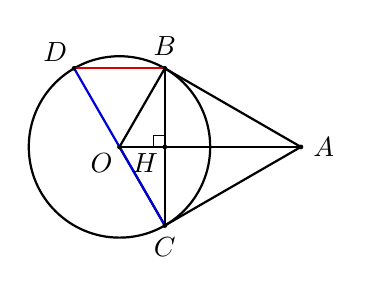
\begin{tikzpicture}[scale=0.72, >=stealth, line join=round, line cap=round]
  \coordinate (O) at (0, 0);
  \coordinate (A) at (3.2, 0);
  \coordinate (B) at (0.8, 1.386);
  \coordinate (C) at (0.8, -1.386);
  \coordinate (D) at (-0.8, 1.386);
  \coordinate (H) at (0.8, 0);
  
  \draw[thick] (O) circle (1.6);
  \draw[thick] (A) -- (B);
  \draw[thick] (A) -- (C);
  \draw[thick] (O) -- (A);
  \draw[thick] (O) -- (B);
  \draw[thick] (O) -- (C);
  \draw[thick] (B) -- (C);
  \draw[thick, blue!85!black] (C) -- (D);
  \draw[thick, red!85!black] (B) -- (D);
  
  \draw (0.8, 0.2) -- (0.6, 0.2) -- (0.6, 0);
  
  \fill (O) circle (1.2pt) node[below left=-1pt] {$O$};
  \fill (A) circle (1.2pt) node[right=1pt] {$A$};
  \fill (B) circle (1.2pt) node[above=1pt] {$B$};
  \fill (C) circle (1.2pt) node[below=1pt] {$C$};
  \fill (D) circle (1.2pt) node[above left=-1pt] {$D$};
  \fill (H) circle (1.2pt) node[below left=-1pt] {$H$};
\end{tikzpicture}
\end{minipage}\par
\vspace{0.4mm}
\noindent\textit{Bài giải:}\dongke{15}
\\ \hline
\end{tabularx}

\newpage
% =============================================================================
% ========================= TOAN 9 TUAN 10 BUOI 01 - MA DE 102 =================
% ========================= TRANG 1/2 ==========================================
% =============================================================================
\noindent
\begin{tabularx}{\linewidth}{|X|c|}
\hline
\textbf{PHIẾU KIỂM TRA ĐỊNH KỲ TOÁN 9 - TUẦN 10 - BUỔI 1} & \textbf{Mã đề: 102 - Trang 1/2} \\
\hline
\end{tabularx}

\vspace{1.0mm}

\noindent
\begin{tabularx}{\linewidth}{|p{3.2cm}|X|}
\hline
\centering\textbf{ĐIỂM SỐ} & \centering\textbf{LỜI NHẬN XÉT CỦA THẦY CÔ} \tabularnewline
\hline
\rule{0pt}{1.8cm} & \tabularnewline
\hline
\end{tabularx}

\vspace{1.2mm}
\noindent\textbf{Câu 1 (0,25 điểm).} Cho $(O; 5\text{ cm})$, khoảng cách $d(O, a) = 3\text{ cm}$. Số điểm chung là: \shortans{2}\par\vspace{0.5mm}
\noindent\textbf{Câu 2 (0,25 điểm).} Tiếp tuyến $Ax$ của $(O)$ tại $A$. Khẳng định đúng là $Ax \dots OA$: \shortans{\perp}\par\vspace{0.5mm}
\noindent\textbf{Câu 3 (0,25 điểm).} Cho $(O; 5\text{ cm}), OA = 13\text{ cm}$, tiếp tuyến $AB$ ($B \in (O)$). Độ dài $AB$ là: \shortans{12\text{ cm}}\par\vspace{0.5mm}
\noindent\textbf{Câu 4 (0,25 điểm).} Căn bậc hai số học của $144$ là: \shortans{12}\par\vspace{0.5mm}
\noindent\textbf{Câu 5 (0,25 điểm).} Điều kiện xác định của biểu thức $\sqrt{4x - 16}$ là: \shortans{x \ge 4}\par\vspace{0.5mm}
\noindent\textbf{Câu 6 (0,25 điểm).} Tính giá trị của biểu thức $\sqrt{48} - \sqrt{27} + \sqrt{12} = $ \shortans{3\sqrt{3}}\par\vspace{0.5mm}
\noindent\textbf{Câu 7 (0,25 điểm).} Hệ phương trình $\begin{cases} 2x + y = 8 \\ x - y = 1 \end{cases}$ có nghiệm $(x; y)$ là: \shortans{(3; 2)}\par\vspace{0.5mm}
\noindent\textbf{Câu 8 (0,25 điểm).} $\Delta$ vuông có đường cao $h$, hai hình chiếu $2\text{ cm}$ và $8\text{ cm}$. Độ dài $h$ là: \shortans{4\text{ cm}}\par\vspace{0.5mm}
\noindent\textbf{Câu 9 (0,25 điểm).} Đường tròn $(O; 10\text{ cm})$, dây $CD = 16\text{ cm}$. Khoảng cách từ $O$ đến $CD$ là: \shortans{6\text{ cm}}\par\vspace{0.5mm}
\noindent\textbf{Câu 10 (0,25 điểm).} Thang dài $6\text{ m}$, chân cách tường $3\text{ m}$. Góc tạo bởi thang và đất là: \shortans{60^\circ}\par\vspace{0.5mm}
\vspace{0.8mm}
\noindent\textbf{Câu 11 (2,5 điểm). Đại số tổng hợp:}
\vspace{0.6mm}

\noindent
\begin{tabularx}{\linewidth}{|X|X|}
\hline
\oBaiTap[19]{a) (1,25 điểm)}{Giải hệ phương trình: $\begin{cases} \dfrac{3}{x + 1} + \dfrac{2}{y - 1} = 5 \\ \dfrac{1}{x + 1} - \dfrac{1}{y - 1} = 0 \end{cases}$} & 
\oBaiTap[19]{b) (1,25 điểm)}{Cho $P = \left( \dfrac{\sqrt{x}}{\sqrt{x} - 2} - \dfrac{4}{x - 2\sqrt{x}} \right) : \dfrac{\sqrt{x} + 2}{x - 4}$ ($x > 0, x \ne 4$). Rút gọn $P$ và tính $P$ tại $x = 16$.} \\
\hline
\end{tabularx}

\newpage
% =============================================================================
% ========================= TOAN 9 TUAN 10 BUOI 01 - MA DE 102 =================
% ========================= TRANG 2/2 ==========================================
% =============================================================================
\noindent
\begin{tabularx}{\linewidth}{|X|c|}
\hline
\textbf{TOÁN 9 - TUẦN 10 - BUỔI 1} & \textbf{Mã đề: 102 - Trang 2/2} \\
\hline
\end{tabularx}

\vspace{1.2mm}

\noindent
\begin{tabularx}{\linewidth}{|X|}
\hline
\vspace{0.5mm}
\textbf{Câu 12 (2,5 điểm).} Một ca nô chạy trên khúc sông trong $4$ giờ, xuôi dòng $90\text{ km}$ và ngược dòng $32\text{ km}$. Một lần khác ca nô đó cũng chạy trong $4$ giờ, xuôi dòng $60\text{ km}$ và ngược dòng $48\text{ km}$. Tính vận tốc thực của ca nô và vận tốc dòng nước (biết các vận tốc không đổi).\par
\vspace{0.4mm}
\noindent\textit{Bài giải:}\dongke{15}
\\ \hline
\end{tabularx}

\vspace{1.2mm}

\noindent
\begin{tabularx}{\linewidth}{|X|}
\hline
\vspace{0.5mm}
\begin{minipage}[t]{0.68\linewidth}
\vspace{0pt}
\textbf{Câu 13 (2,5 điểm).} Cho đường tròn $(O; R)$ và điểm $A$ nằm bên ngoài đường tròn. Qua $A$ kẻ tiếp tuyến $AB$ với đường tròn $(O)$ ($B$ là tiếp điểm). Kẻ dây $BC \perp OA$ tại $H$ ($C \ne B$).\par\vspace{0.4mm}
\textbf{a) (1,25 điểm)} Chứng minh đường thẳng $AC$ là tiếp tuyến của đường tròn $(O)$.\par\vspace{0.4mm}
\textbf{b) (1,25 điểm)} Kẻ đường kính $CD$ của $(O)$. Chứng minh $BD \parallel OA$. Cho $R = 6\text{ cm}, OA = 10\text{ cm}$, tính độ dài $BC$.
\end{minipage}\hfill
\begin{minipage}[t]{0.30\linewidth}
\vspace{0pt}\centering
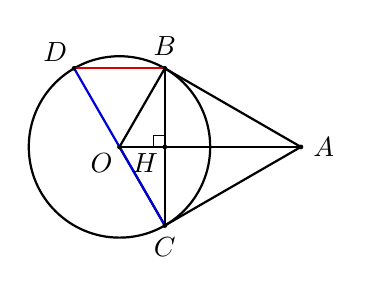
\begin{tikzpicture}[scale=0.72, >=stealth, line join=round, line cap=round]
  \coordinate (O) at (0, 0);
  \coordinate (A) at (3.2, 0);
  \coordinate (B) at (0.8, 1.386);
  \coordinate (C) at (0.8, -1.386);
  \coordinate (D) at (-0.8, 1.386);
  \coordinate (H) at (0.8, 0);
  
  \draw[thick] (O) circle (1.6);
  \draw[thick] (A) -- (B);
  \draw[thick] (A) -- (C);
  \draw[thick] (O) -- (A);
  \draw[thick] (O) -- (B);
  \draw[thick] (O) -- (C);
  \draw[thick] (B) -- (C);
  \draw[thick, blue!85!black] (C) -- (D);
  \draw[thick, red!85!black] (B) -- (D);
  
  \draw (0.8, 0.2) -- (0.6, 0.2) -- (0.6, 0);
  
  \fill (O) circle (1.2pt) node[below left=-1pt] {$O$};
  \fill (A) circle (1.2pt) node[right=1pt] {$A$};
  \fill (B) circle (1.2pt) node[above=1pt] {$B$};
  \fill (C) circle (1.2pt) node[below=1pt] {$C$};
  \fill (D) circle (1.2pt) node[above left=-1pt] {$D$};
  \fill (H) circle (1.2pt) node[below left=-1pt] {$H$};
\end{tikzpicture}
\end{minipage}\par
\vspace{0.4mm}
\noindent\textit{Bài giải:}\dongke{15}
\\ \hline
\end{tabularx}

\newpage
% =============================================================================
% ========================= TOAN 9 TUAN 10 BUOI 01 - MA DE 103 =================
% ========================= TRANG 1/2 ==========================================
% =============================================================================
\noindent
\begin{tabularx}{\linewidth}{|X|c|}
\hline
\textbf{PHIẾU KIỂM TRA ĐỊNH KỲ TOÁN 9 - TUẦN 10 - BUỔI 1} & \textbf{Mã đề: 103 - Trang 1/2} \\
\hline
\end{tabularx}

\vspace{1.0mm}

\noindent
\begin{tabularx}{\linewidth}{|p{3.2cm}|X|}
\hline
\centering\textbf{ĐIỂM SỐ} & \centering\textbf{LỜI NHẬN XÉT CỦA THẦY CÔ} \tabularnewline
\hline
\rule{0pt}{1.8cm} & \tabularnewline
\hline
\end{tabularx}

\vspace{1.2mm}
\noindent\textbf{Câu 1 (0,25 điểm).} Cho $(O; 6\text{ cm})$, khoảng cách $d(O, a) = 7\text{ cm}$. Số điểm chung là: \shortans{0}\par\vspace{0.5mm}
\noindent\textbf{Câu 2 (0,25 điểm).} Tiếp tuyến của $(O)$ vuông góc với bán kính đi qua điểm nào: \shortans{\text{tiếp điểm}}\par\vspace{0.5mm}
\noindent\textbf{Câu 3 (0,25 điểm).} Cho $(O; 6\text{ cm}), OA = 10\text{ cm}$, tiếp tuyến $AB$ ($B \in (O)$). Độ dài $AB$ là: \shortans{8\text{ cm}}\par\vspace{0.5mm}
\noindent\textbf{Câu 4 (0,25 điểm).} Căn bậc hai số học của $169$ là: \shortans{13}\par\vspace{0.5mm}
\noindent\textbf{Câu 5 (0,25 điểm).} Điều kiện xác định của biểu thức $\sqrt{5x - 15}$ là: \shortans{x \ge 3}\par\vspace{0.5mm}
\noindent\textbf{Câu 6 (0,25 điểm).} Tính giá trị của biểu thức $\sqrt{50} - \sqrt{32} + \sqrt{18} = $ \shortans{4\sqrt{2}}\par\vspace{0.5mm}
\noindent\textbf{Câu 7 (0,25 điểm).} Hệ phương trình $\begin{cases} 2x + y = 9 \\ x - y = 3 \end{cases}$ có nghiệm $(x; y)$ là: \shortans{(4; 1)}\par\vspace{0.5mm}
\noindent\textbf{Câu 8 (0,25 điểm).} $\Delta$ vuông có đường cao $h$, hai hình chiếu $3\text{ cm}$ và $12\text{ cm}$. Độ dài $h$ là: \shortans{6\text{ cm}}\par\vspace{0.5mm}
\noindent\textbf{Câu 9 (0,25 điểm).} Đường tròn $(O; 13\text{ cm})$, dây $CD = 24\text{ cm}$. Khoảng cách từ $O$ đến $CD$ là: \shortans{5\text{ cm}}\par\vspace{0.5mm}
\noindent\textbf{Câu 10 (0,25 điểm).} Cột cờ cao $5\text{ m}$, bóng trên đất dài $5\text{ m}$. Góc tia nắng với mặt đất là: \shortans{45^\circ}\par\vspace{0.5mm}
\vspace{0.8mm}
\noindent\textbf{Câu 11 (2,5 điểm). Đại số tổng hợp:}
\vspace{0.6mm}

\noindent
\begin{tabularx}{\linewidth}{|X|X|}
\hline
\oBaiTap[19]{a) (1,25 điểm)}{Giải hệ phương trình: $\begin{cases} \dfrac{2}{x - 2} + \dfrac{3}{y + 1} = 5 \\ \dfrac{4}{x - 2} - \dfrac{1}{y + 1} = 3 \end{cases}$} & 
\oBaiTap[19]{b) (1,25 điểm)}{Cho $P = \left( \dfrac{\sqrt{x}}{\sqrt{x} - 3} - \dfrac{9}{x - 3\sqrt{x}} \right) : \dfrac{\sqrt{x} + 3}{x - 9}$ ($x > 0, x \ne 9$). Rút gọn $P$ và tính $P$ tại $x = 4$.} \\
\hline
\end{tabularx}

\newpage
% =============================================================================
% ========================= TOAN 9 TUAN 10 BUOI 01 - MA DE 103 =================
% ========================= TRANG 2/2 ==========================================
% =============================================================================
\noindent
\begin{tabularx}{\linewidth}{|X|c|}
\hline
\textbf{TOÁN 9 - TUẦN 10 - BUỔI 1} & \textbf{Mã đề: 103 - Trang 2/2} \\
\hline
\end{tabularx}

\vspace{1.2mm}

\noindent
\begin{tabularx}{\linewidth}{|X|}
\hline
\vspace{0.5mm}
\textbf{Câu 12 (2,5 điểm).} Một ca nô chạy trên khúc sông trong $5$ giờ, xuôi dòng $60\text{ km}$ và ngược dòng $48\text{ km}$. Một lần khác ca nô đó cũng chạy trong $5$ giờ, xuôi dòng $40\text{ km}$ và ngược dòng $64\text{ km}$. Tính vận tốc thực của ca nô và vận tốc dòng nước (biết các vận tốc không đổi).\par
\vspace{0.4mm}
\noindent\textit{Bài giải:}\dongke{15}
\\ \hline
\end{tabularx}

\vspace{1.2mm}

\noindent
\begin{tabularx}{\linewidth}{|X|}
\hline
\vspace{0.5mm}
\begin{minipage}[t]{0.68\linewidth}
\vspace{0pt}
\textbf{Câu 13 (2,5 điểm).} Cho đường tròn $(O; R)$ và điểm $A$ nằm bên ngoài đường tròn. Qua $A$ kẻ tiếp tuyến $AB$ với đường tròn $(O)$ ($B$ là tiếp điểm). Kẻ dây $BC \perp OA$ tại $H$ ($C \ne B$).\par\vspace{0.4mm}
\textbf{a) (1,25 điểm)} Chứng minh đường thẳng $AC$ là tiếp tuyến của đường tròn $(O)$.\par\vspace{0.4mm}
\textbf{b) (1,25 điểm)} Kẻ đường kính $CD$ của $(O)$. Chứng minh $BD \parallel OA$. Cho $R = 9\text{ cm}, OA = 15\text{ cm}$, tính độ dài $BC$.
\end{minipage}\hfill
\begin{minipage}[t]{0.30\linewidth}
\vspace{0pt}\centering
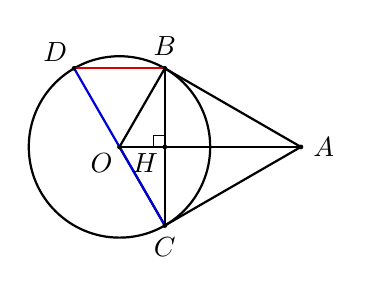
\begin{tikzpicture}[scale=0.72, >=stealth, line join=round, line cap=round]
  \coordinate (O) at (0, 0);
  \coordinate (A) at (3.2, 0);
  \coordinate (B) at (0.8, 1.386);
  \coordinate (C) at (0.8, -1.386);
  \coordinate (D) at (-0.8, 1.386);
  \coordinate (H) at (0.8, 0);
  
  \draw[thick] (O) circle (1.6);
  \draw[thick] (A) -- (B);
  \draw[thick] (A) -- (C);
  \draw[thick] (O) -- (A);
  \draw[thick] (O) -- (B);
  \draw[thick] (O) -- (C);
  \draw[thick] (B) -- (C);
  \draw[thick, blue!85!black] (C) -- (D);
  \draw[thick, red!85!black] (B) -- (D);
  
  \draw (0.8, 0.2) -- (0.6, 0.2) -- (0.6, 0);
  
  \fill (O) circle (1.2pt) node[below left=-1pt] {$O$};
  \fill (A) circle (1.2pt) node[right=1pt] {$A$};
  \fill (B) circle (1.2pt) node[above=1pt] {$B$};
  \fill (C) circle (1.2pt) node[below=1pt] {$C$};
  \fill (D) circle (1.2pt) node[above left=-1pt] {$D$};
  \fill (H) circle (1.2pt) node[below left=-1pt] {$H$};
\end{tikzpicture}
\end{minipage}\par
\vspace{0.4mm}
\noindent\textit{Bài giải:}\dongke{15}
\\ \hline
\end{tabularx}

\newpage
% =============================================================================
% ========================= TOAN 9 TUAN 10 BUOI 01 - MA DE 104 =================
% ========================= TRANG 1/2 ==========================================
% =============================================================================
\noindent
\begin{tabularx}{\linewidth}{|X|c|}
\hline
\textbf{PHIẾU KIỂM TRA ĐỊNH KỲ TOÁN 9 - TUẦN 10 - BUỔI 1} & \textbf{Mã đề: 104 - Trang 1/2} \\
\hline
\end{tabularx}

\vspace{1.0mm}

\noindent
\begin{tabularx}{\linewidth}{|p{3.2cm}|X|}
\hline
\centering\textbf{ĐIỂM SỐ} & \centering\textbf{LỜI NHẬN XÉT CỦA THẦY CÔ} \tabularnewline
\hline
\rule{0pt}{1.8cm} & \tabularnewline
\hline
\end{tabularx}

\vspace{1.2mm}
\noindent\textbf{Câu 1 (0,25 điểm).} Cho $(O; 5\text{ cm})$, đường thẳng $d$ tiếp xúc với $(O)$. Khoảng cách từ $O$ đến $d$ là: \shortans{5\text{ cm}}\par\vspace{0.5mm}
\noindent\textbf{Câu 2 (0,25 điểm).} Nếu đường thẳng $d \perp OA$ tại $A \in (O)$ thì $d$ được gọi là: \shortans{\text{tiếp tuyến}}\par\vspace{0.5mm}
\noindent\textbf{Câu 3 (0,25 điểm).} Cho $(O; 8\text{ cm}), OA = 17\text{ cm}$, tiếp tuyến $AB$ ($B \in (O)$). Độ dài $AB$ là: \shortans{15\text{ cm}}\par\vspace{0.5mm}
\noindent\textbf{Câu 4 (0,25 điểm).} Căn bậc hai số học của $196$ là: \shortans{14}\par\vspace{0.5mm}
\noindent\textbf{Câu 5 (0,25 điểm).} Điều kiện xác định của biểu thức $\sqrt{2x - 10}$ là: \shortans{x \ge 5}\par\vspace{0.5mm}
\noindent\textbf{Câu 6 (0,25 điểm).} Tính giá trị của biểu thức $\sqrt{75} - \sqrt{27} + \sqrt{12} = $ \shortans{4\sqrt{3}}\par\vspace{0.5mm}
\noindent\textbf{Câu 7 (0,25 điểm).} Hệ phương trình $\begin{cases} 2x + y = 10 \\ x - y = 2 \end{cases}$ có nghiệm $(x; y)$ là: \shortans{(4; 2)}\par\vspace{0.5mm}
\noindent\textbf{Câu 8 (0,25 điểm).} $\Delta$ vuông có đường cao $h$, hai hình chiếu $1\text{ cm}$ và $9\text{ cm}$. Độ dài $h$ là: \shortans{3\text{ cm}}\par\vspace{0.5mm}
\noindent\textbf{Câu 9 (0,25 điểm).} Đường tròn $(O; 5\text{ cm})$, khoảng cách từ $O$ đến dây $CD$ là $4\text{ cm}$. Độ dài $CD$ là: \shortans{6\text{ cm}}\par\vspace{0.5mm}
\noindent\textbf{Câu 10 (0,25 điểm).} Cọc cao $3\text{ m}$, bóng trên đất dài $3\text{ m}$. Góc tia nắng với mặt đất là: \shortans{45^\circ}\par\vspace{0.5mm}
\vspace{0.8mm}
\noindent\textbf{Câu 11 (2,5 điểm). Đại số tổng hợp:}
\vspace{0.6mm}

\noindent
\begin{tabularx}{\linewidth}{|X|X|}
\hline
\oBaiTap[19]{a) (1,25 điểm)}{Giải hệ phương trình: $\begin{cases} \dfrac{1}{x + 2} + \dfrac{2}{y - 3} = 3 \\ \dfrac{3}{x + 2} - \dfrac{1}{y - 3} = 2 \end{cases}$} & 
\oBaiTap[19]{b) (1,25 điểm)}{Cho $P = \left( \dfrac{\sqrt{x}}{\sqrt{x} - 1} - \dfrac{1}{x - \sqrt{x}} \right) : \dfrac{\sqrt{x} + 1}{x - 1}$ ($x > 0, x \ne 1$). Rút gọn $P$ và tính $P$ tại $x = 25$.} \\
\hline
\end{tabularx}

\newpage
% =============================================================================
% ========================= TOAN 9 TUAN 10 BUOI 01 - MA DE 104 =================
% ========================= TRANG 2/2 ==========================================
% =============================================================================
\noindent
\begin{tabularx}{\linewidth}{|X|c|}
\hline
\textbf{TOÁN 9 - TUẦN 10 - BUỔI 1} & \textbf{Mã đề: 104 - Trang 2/2} \\
\hline
\end{tabularx}

\vspace{1.2mm}

\noindent
\begin{tabularx}{\linewidth}{|X|}
\hline
\vspace{0.5mm}
\textbf{Câu 12 (2,5 điểm).} Một ca nô chạy trên khúc sông trong $6$ giờ, xuôi dòng $90\text{ km}$ và ngược dòng $60\text{ km}$. Một lần khác ca nô đó cũng chạy trong $6$ giờ, xuôi dòng $120\text{ km}$ và ngược dòng $40\text{ km}$. Tính vận tốc thực của ca nô và vận tốc dòng nước (biết các vận tốc không đổi).\par
\vspace{0.4mm}
\noindent\textit{Bài giải:}\dongke{15}
\\ \hline
\end{tabularx}

\vspace{1.2mm}

\noindent
\begin{tabularx}{\linewidth}{|X|}
\hline
\vspace{0.5mm}
\begin{minipage}[t]{0.68\linewidth}
\vspace{0pt}
\textbf{Câu 13 (2,5 điểm).} Cho đường tròn $(O; R)$ và điểm $A$ nằm bên ngoài đường tròn. Qua $A$ kẻ tiếp tuyến $AB$ với đường tròn $(O)$ ($B$ là tiếp điểm). Kẻ dây $BC \perp OA$ tại $H$ ($C \ne B$).\par\vspace{0.4mm}
\textbf{a) (1,25 điểm)} Chứng minh đường thẳng $AC$ là tiếp tuyến của đường tròn $(O)$.\par\vspace{0.4mm}
\textbf{b) (1,25 điểm)} Kẻ đường kính $CD$ của $(O)$. Chứng minh $BD \parallel OA$. Cho $R = 12\text{ cm}, OA = 20\text{ cm}$, tính độ dài $BC$.
\end{minipage}\hfill
\begin{minipage}[t]{0.30\linewidth}
\vspace{0pt}\centering
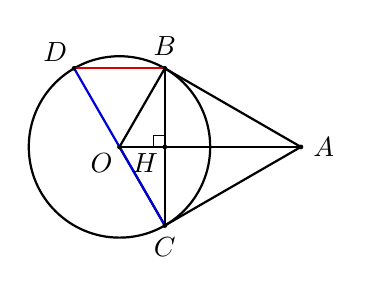
\begin{tikzpicture}[scale=0.72, >=stealth, line join=round, line cap=round]
  \coordinate (O) at (0, 0);
  \coordinate (A) at (3.2, 0);
  \coordinate (B) at (0.8, 1.386);
  \coordinate (C) at (0.8, -1.386);
  \coordinate (D) at (-0.8, 1.386);
  \coordinate (H) at (0.8, 0);
  
  \draw[thick] (O) circle (1.6);
  \draw[thick] (A) -- (B);
  \draw[thick] (A) -- (C);
  \draw[thick] (O) -- (A);
  \draw[thick] (O) -- (B);
  \draw[thick] (O) -- (C);
  \draw[thick] (B) -- (C);
  \draw[thick, blue!85!black] (C) -- (D);
  \draw[thick, red!85!black] (B) -- (D);
  
  \draw (0.8, 0.2) -- (0.6, 0.2) -- (0.6, 0);
  
  \fill (O) circle (1.2pt) node[below left=-1pt] {$O$};
  \fill (A) circle (1.2pt) node[right=1pt] {$A$};
  \fill (B) circle (1.2pt) node[above=1pt] {$B$};
  \fill (C) circle (1.2pt) node[below=1pt] {$C$};
  \fill (D) circle (1.2pt) node[above left=-1pt] {$D$};
  \fill (H) circle (1.2pt) node[below left=-1pt] {$H$};
\end{tikzpicture}
\end{minipage}\par
\vspace{0.4mm}
\noindent\textit{Bài giải:}\dongke{15}
\\ \hline
\end{tabularx}
\end{document}
